\documentclass[a4paper,11pt,twoside]{exam}


\noprintanswers % Pour ne pas imprimer les réponses (énoncé)
% \printanswers % pour imprimer les réponses (corrigé)


% \addpoints % Pour compter les points
% \noaddpoints % pour ne pas compter les points
% \qformat{\textbf{Question\thequestion}\quad(\thepoints)\hfill} % Pour définir le style des questions (facultatif)
\usepackage{color} % définit une nouvelle couleur

\shadedsolutions % définit le style des réponses
% \framedsolutions % définit le style des réponses
\definecolor{SolutionColor}{rgb}{0.8,0.9,1} % bleu ciel
\renewcommand{\solutiontitle}{\noindent\textbf{Solution:}\par\noindent} % Définit le titre des solutions

\newcommand{\titrecours}{HMMA 237 -- Séries Temporelles Avancées
}
\newcommand{\numsession}{1}
\newcommand{\annee}{2018/2019}
\newcommand{\ecole}{Universit\'e de Montpellier}
\newcommand{\dateexam}{Universit\'e de Montpellier}
\newcommand{\duree}{2h}
\newcommand{\documentok}{Aucun}
\newcommand{\materielok}{Aucun}

\usepackage{../sty/examens} % locate examens.sty
\usepackage{../sty/shortcuts_js} % locate shortcuts_js.sty

% Logo images in prebuiltimages/


\usepackage{tikz}
\usetikzlibrary{arrows}



\begin{document}
\sloppy
\myheader

\begin{center}
\textbf{Le soin apporté à la rédaction sera un élément important d'appréciation.}
\end{center}
% \textbf{Un formulaire est disponible à la fin du sujet et peut-être réutilisé à loisir.}
\begin{center}
\bigskip
\underline{\large \textbf{Questions de cours}} % (5 points)
\end{center}

\begin{enumerate}[label=QdC - \arabic*.]
    \item Rappeler la définition de l'estimateur Ridge comme solution d'un problème de minimisation.
    On pourra noter $X \in \bbR^{n\times p}$ la matrice des variables explicatives, et $y\in \bbR^n$ le signal observé.
    Donner également une formule explicite de cet estimateur.

    \begin{solution}(1pt)
    \begin{align*}
        \hat\beta \in \argmin_{\beta \in \bbR^p} \norm{y - X \beta}^2 + \lambda \norm{\beta}^2_2\enspace,
    \end{align*} et $\hat\beta = (X^\top X + \lambda \Id_p)^{-1} X^\top y$.
    \end{solution}
    \item Donner la formule de mise à jour pour effectuer une étape de descente de gradient (avec un pas $\alpha$) afin de minimiser la fonction
\end{enumerate}

%%%%%%%%%%%%%%%%%%%%%%%%%%%%%%%%%%%%%%%%%%%%%%%%%%%%%%%%%%%%%%%%%%%%%%%%%%%%%%%
\begin{exercice} % (??? points)
Soit $G = (V,E)$ un graphe (non-orienté) à $n$ sommets, $V = \llbracket 1,n \rrbracket $, et $p$ arrêtes, $E = \llbracket 1, p\rrbracket$.
Le graphe peut être représenté par sa matrice d'incidence arrête-sommet $D^\top \in \mathbb{R}^{p \times n}$ définie par
\begin{equation}
  (D^\top)_{e,v} =
  \begin{cases}
    + 1, & \text{si } v = \min(i,j), \\
    - 1, & \text{si } v = \max(i,j),  \\
    0, & \text{sinon}.
  \end{cases}
\end{equation}
où $e = \{i,j\}$.

\begin{enumerate}[label=\Roman{numeroexo} - \arabic*.]
    \item Dans le graphe décrit en Figure~\ref{fig:graphAtoG}, trouver le plus court chemin pour aller de $A$ vers $G$.
    \begin{solution}(1pt)
        $A\to B \to C' \to D'\to E \to F' \to G$
    \end{solution}
    \begin{figure}[h]
\centering
\small
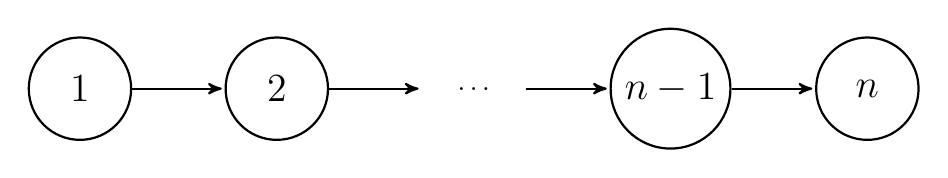
\begin{tikzpicture}[->,>=stealth',shorten >=1pt,auto,node distance=2.5cm,
                    thick,main node/.style={circle,draw,font=\sffamily\Large\bfseries}]

  \node[main node,minimum size=1.3cm] (1) {$1$};
  \node[main node,minimum size=1.3cm] (2) [right of=1] {$2$};
  \node[fill=none,minimum size=1.3cm] (3) [right of=2] {$\dots$};
  \node[main node,minimum size=1.3cm] (4) [right of=3] {$n-1$};
  \node[main node,minimum size=1.3cm] (5) [right of=4] {$n$};


  \path[every node/.style={font=\sffamily}] % \small
    (1) edge node [left] {} (2)

    (2) edge node [left] {} (3)

    % (3) edge node [left] {} (4)

    (4) edge node [above] {} (5)
    ;
    \draw (3) -- (4);
\end{tikzpicture}
\caption{Graphe en ligne avec des arêtes non-pondérées.}
\label{fig:graph_ligne}
\end{figure}


\begin{figure}[h]
\centering
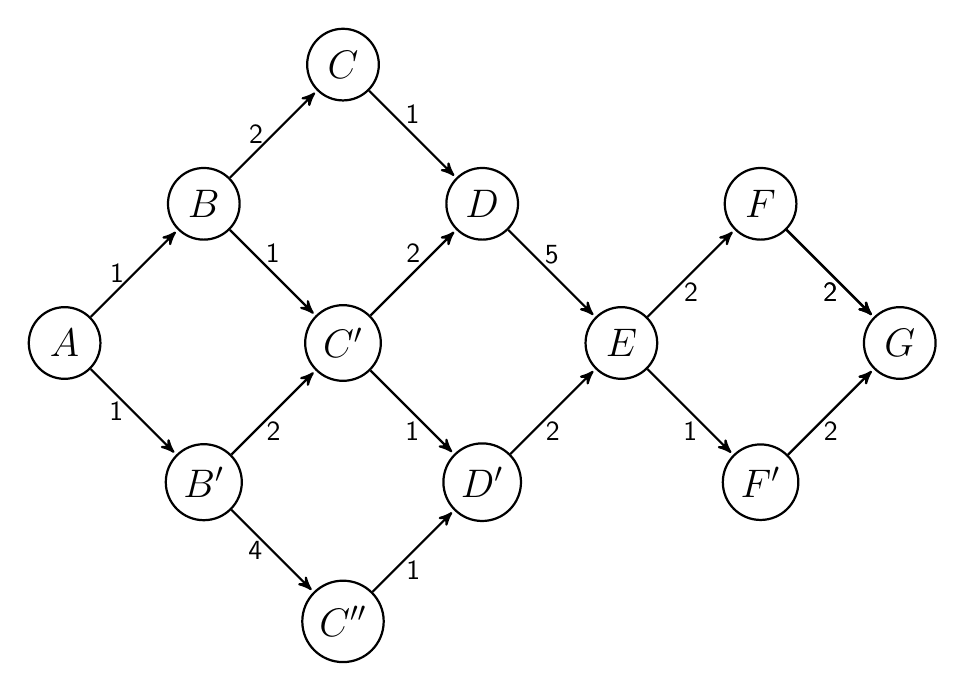
\begin{tikzpicture}[->,>=stealth',shorten >=1pt,auto,node distance=2.5cm,
                    thick,main node/.style={circle,draw,font=\sffamily\Large\bfseries}]

  \node[main node,minimum size=0.91cm] (1) {$A$};
  \node[main node,minimum size=0.91cm] (2) [above right of=1] {$B$};
  \node[main node,minimum size=0.91cm] (3) [below right of=1] {$B'$};
  \node[main node,minimum size=0.91cm] (4) [above right of=2] {$C$};
  \node[main node,minimum size=0.91cm] (5) [below right of=2] {$C'$};
  \node[main node,minimum size=0.91cm] (6) [below right of=3] {$C''$};
  \node[main node,minimum size=0.91cm] (7) [below right of=4] {$D$};
  \node[main node,minimum size=0.91cm] (8) [below right of=5] {$D'$};
  \node[main node,minimum size=0.91cm] (9) [below right of=7] {$E$};
  \node[main node,minimum size=0.91cm] (10) [above right of=9] {$F$};
  \node[main node,minimum size=0.91cm] (11) [below right of=9] {$F'$};
  \node[main node,minimum size=0.91cm] (12) [below right of=10] {$G$};


  \path[every node/.style={font=\sffamily}] % \small
    (1) edge node [left] {1} (2)
        edge node [left] {1} (3)

    (2) edge node [left] {2} (4)
        edge node [above] {1} (5)

    (3) edge node [below] {2} (5)
        edge node [left] {4} (6)

    (4) edge node [above] {1} (7)

    (5) edge node [above] {2} (7)
        edge node [below] {1} (8)

    (6) edge node [below] {1} (8)

    (7) edge node [above] {5} (9)

    (8) edge node [below] {2} (9)

    (9) edge node [below] {2} (10)
        edge node [below] {1} (11)

    (10) edge node [below] {2} (12)
    (10) edge node [below] {2} (12)
    (11) edge node [below] {2} (12)

    ;
\end{tikzpicture}
\caption{Graphe de A à G avec des arêtes pondérées.}
\label{fig:graphAtoG}
\end{figure}
\end{enumerate}
Dans la suite on ne considère plus que des graphes non orientés sans poids: on négligera les ``flèches'' et les poids des arrêtes.
\begin{enumerate}[resume,label=\Roman{numeroexo} - \arabic*.]
    \item Pour les graphes donnés en Figure~\ref{fig:graph_ligne} et \ref{fig:graphAtoG}, calculer la matrice d'incidence $D^\top$ décrite ci-dessus ainsi que la matrice $L = D D^\top \in \bbR^{n \times n}$.

    \begin{solution}(2pt)
    {\small
    \setcounter{MaxMatrixCols}{20}
    \begin{align*}
    D^\top =
        \begin{pmatrix}
        -1 &  1 &  0 &  0 &  0 &  0 &  0 &  0 &  0 &  0 &  0 &  0 \\
        -1 &  0 &  1 &  0 &  0 &  0 &  0 &  0 &  0 &  0 &  0 &  0 \\
         0 & -1 &  0 &  1 &  0 &  0 &  0 &  0 &  0 &  0 &  0 &  0 \\
         0 & -1 &  0 &  0 &  1 &  0 &  0 &  0 &  0 &  0 &  0 &  0 \\
         0 &  0 & -1 &  0 &  1 &  0 &  0 &  0 &  0 &  0 &  0 &  0 \\
         0 &  0 & -1 &  0 &  0 &  1 &  0 &  0 &  0 &  0 &  0 &  0 \\
         0 &  0 &  0 & -1 &  0 &  0 &  1 &  0 &  0 &  0 &  0 &  0 \\
         0 &  0 &  0 &  0 & -1 &  0 &  1 &  0 &  0 &  0 &  0 &  0 \\
         0 &  0 &  0 &  0 & -1 &  0 &  0 &  1 &  0 &  0 &  0 &  0 \\
         0 &  0 &  0 &  0 &  0 & -1 &  0 &  1 &  0 &  0 &  0 &  0 \\
         0 &  0 &  0 &  0 &  0 &  0 & -1 &  0 &  1 &  0 &  0 &  0 \\
         0 &  0 &  0 &  0 &  0 &  0 &  0 & -1 &  1 &  0 &  0 &  0 \\
         0 &  0 &  0 &  0 &  0 &  0 &  0 &  0 & -1 &  1 &  0 &  0 \\
         0 &  0 &  0 &  0 &  0 &  0 &  0 &  0 & -1 &  0 &  1 &  0 \\
         0 &  0 &  0 &  0 &  0 &  0 &  0 &  0 &  0 & -1 &  0 &  1 \\
         0 &  0 &  0 &  0 &  0 &  0 &  0 &  0 &  0 &  0 & -1 &  1 \\
        \end{pmatrix}
    \end{align*}}
    De plus
    \begin{align*}
        L=
        \begin{pmatrix}
        & 2 & -1 & -1 &  0 &  0 &  0 &  0 &  0 &  0 &  0 &  0 &  0 \\
        &-1 &  3 &  0 & -1 & -1 &  0 &  0 &  0 &  0 &  0 &  0 &  0 \\
        &-1 &  0 &  3 &  0 & -1 & -1 &  0 &  0 &  0 &  0 &  0 &  0 \\
        & 0 & -1 &  0 &  2 &  0 &  0 & -1 &  0 &  0 &  0 &  0 &  0 \\
        & 0 & -1 & -1 &  0 &  4 &  0 & -1 & -1 &  0 &  0 &  0 &  0 \\
        & 0 &  0 & -1 &  0 &  0 &  2 &  0 & -1 &  0 &  0 &  0 &  0 \\
        & 0 &  0 &  0 & -1 & -1 &  0 &  3 &  0 & -1 &  0 &  0 &  0 \\
        & 0 &  0 &  0 &  0 & -1 & -1 &  0 &  3 & -1 &  0 &  0 &  0 \\
        & 0 &  0 &  0 &  0 &  0 &  0 & -1 & -1 &  4 & -1 & -1 &  0 \\
        & 0 &  0 &  0 &  0 &  0 &  0 &  0 &  0 & -1 &  2 &  0 & -1 \\
        & 0 &  0 &  0 &  0 &  0 &  0 &  0 &  0 & -1 &  0 &  2 & -1 \\
        & 0 &  0 &  0 &  0 &  0 &  0 &  0 &  0 &  0 & -1 & -1 &  2
        \end{pmatrix}
    \end{align*}
    \begin{align*}
    D^\top=
    \begin{bmatrix}
    -1 & 1  &    &                       &                       &    &   \\
       & -1 & 1  &                       &                       &    &   \\
       &    & -1 & 1                     &                       &    &   \\
       &    &    & \ddots                & \ddots                &    &   \\
       &    &    &                       & -1                    & 1  &   \\
       &    &    &                       &                       & -1 & 1
   \end{bmatrix}\in\bbR^{(n-1) \times n}
    \end{align*}
    \begin{align*}
    L=
    \begin{bmatrix}
        1  & -1 &        &       & \\
        -1 & 2  & -1     &       & \\
           & -1 & \ddots & -1    & \\
           &    & -1     & 2 & -1  \\
           &    &        & -1    & n
    \end{bmatrix}\in\bbR^{n \times n}
    \end{align*}
    \end{solution}

    \item Pour un graphe général, déterminer les valeurs des éléments de la matrice $L$, notamment en fonction des degré des sommets, où le degré d'un sommet est le nombre de sommets qui lui sont reliés par une arrête (sans préjugé de la direction). Ainsi, pour tout $v\in V$, $\deg(v) = |\{v' \in V: (v,v') \in E \text{ ou } (v',v) \in E \}|$.
 \end{enumerate}
\end{exercice}
%%%%%%%%%%%%%%%%%%%%%%%%%%%%%%%%%%%%%%%%%%%%%%%%%%%%%%%%%%%%%%%%%%%%%%%%%%%%%%%


\end{document}


